\chapter{Analisi dei risultati}

I grafici presentati sono il frutto delle simulazioni descritte precedentemente. Queste si dividono in quattro sezioni:

\begin{itemize}
 \item Analisi del caso in cui il Front-end abbia distribuzione esponenziale;
 \item Analisi del caso in cui il Front-end ha distribuzione 10 Erlang;
 \item Analisi del caso in cui il Front-end ha distribuzione iperesponenziale;
 \item Analisi del caso peggiore tra i tre sopra descritti con l'overload manager attivo.
\end{itemize}

\noindent Per ognuno di questi sono riportati i dati relativi a:
\begin{enumerate}
 \item Tempo di risposta medio del sistema;
 \item Throughput;
 \item Autocorrelazione.
\end{enumerate}

\section{Front server esponenziale}

\subsection{Tempo di risposta}
Per prima cosa analizziamo il tempo medio di risposta del sistema. Nella figura è rappresentato un grafico con i tempi medi ottenuti ogni 100 secondi di simulazione. Il sistema risulta essere \textbf{instabile}, in quanto i tempi crescono in modo praticamente lineare, questo risulta essere conseguenza del fatto che la cosa del Front server tende a crescere all'infinito.

\begin{figure}[H]
	\begin{center}
	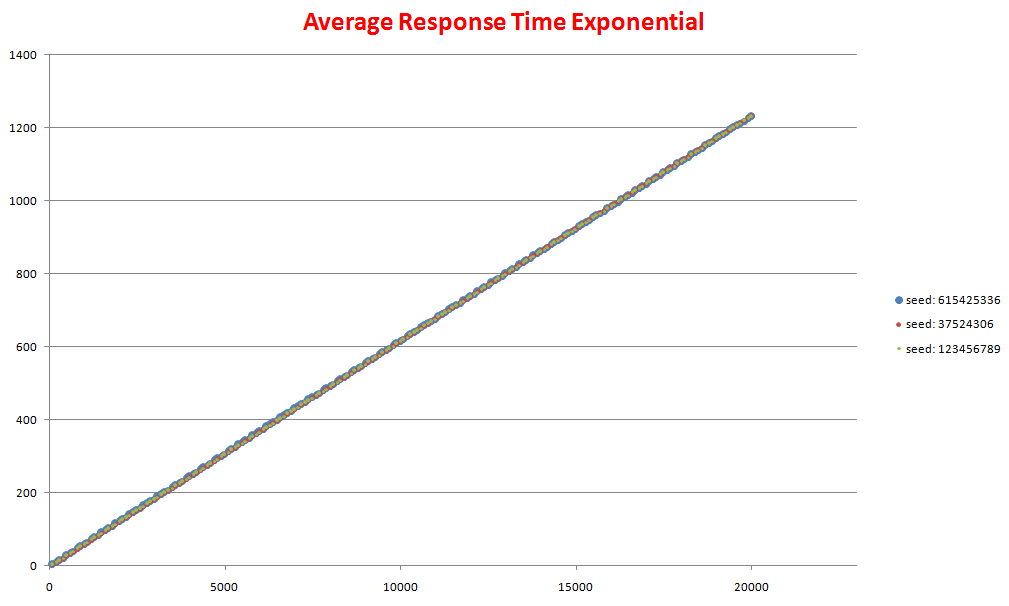
\includegraphics[scale=0.4]{img/exp_res_time.png}
	\caption[Tempo di risposta del sistema senza Overload Management (Legge Front-End:Esponenziale)]{Tempo di risposta del sistema nel caso di tempo di servizio esponenziale senza Overload Management.}
	\label{fig:exp_res_time}
	\end{center}
\end{figure}

\subsection{Throughput}
\begin{figure}[H]
	\begin{center}
	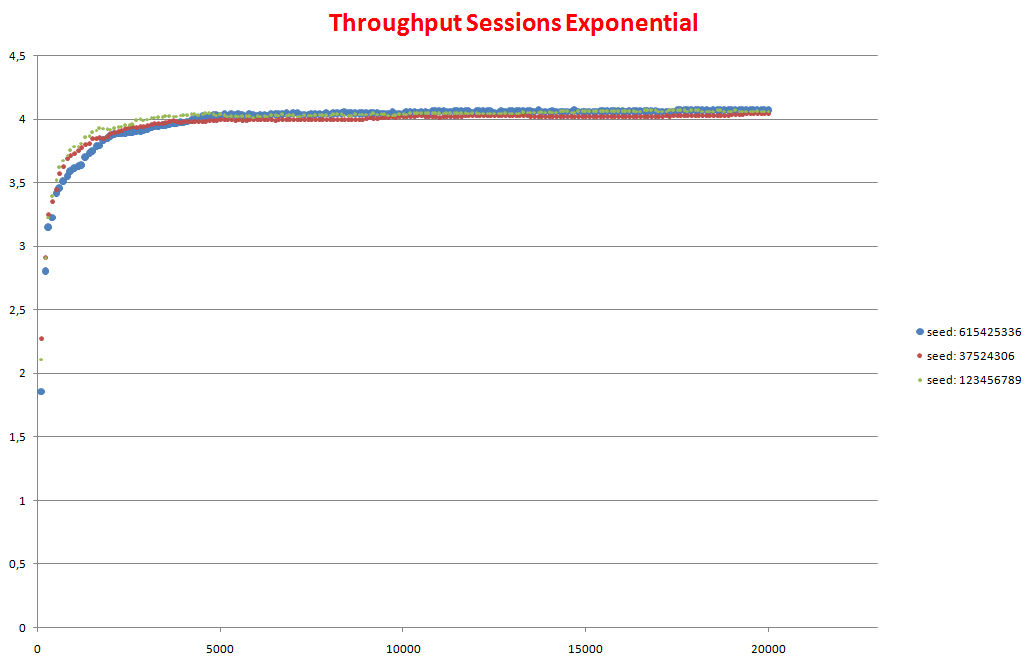
\includegraphics[scale=0.4]{img/exp_t_sess.png}
	\caption[Throughput del sistema senza Overload Management (Legge Front-End:Esponenziale)]{Througput del sistema nel caso di tempo di servizio esponenziale senza Overload Management.}
	\label{fig:exp_t_sess}
	\end{center}
\end{figure}
La seconda metrica di cui ci andiamo ad interessare è quella relativa al throughput. Come si evince dall'immagine c'è una saturazione molto veloce del front-end e infatti questo si stabilizza molto velocemente attorno al valore 4.

Un intervallo di confidenza per il throughput calcolato è il seguente:

\begin{center} IC = [3.96532859 - 0.02472767 ; 3.96532859 - 0.02472767] =  [3.94060091 ; 3.99005626]\end{center}

Mentre qui di seguito vediamo l'istogramma relativo a tale metrica:
\begin{figure}[H]
	\begin{center}
	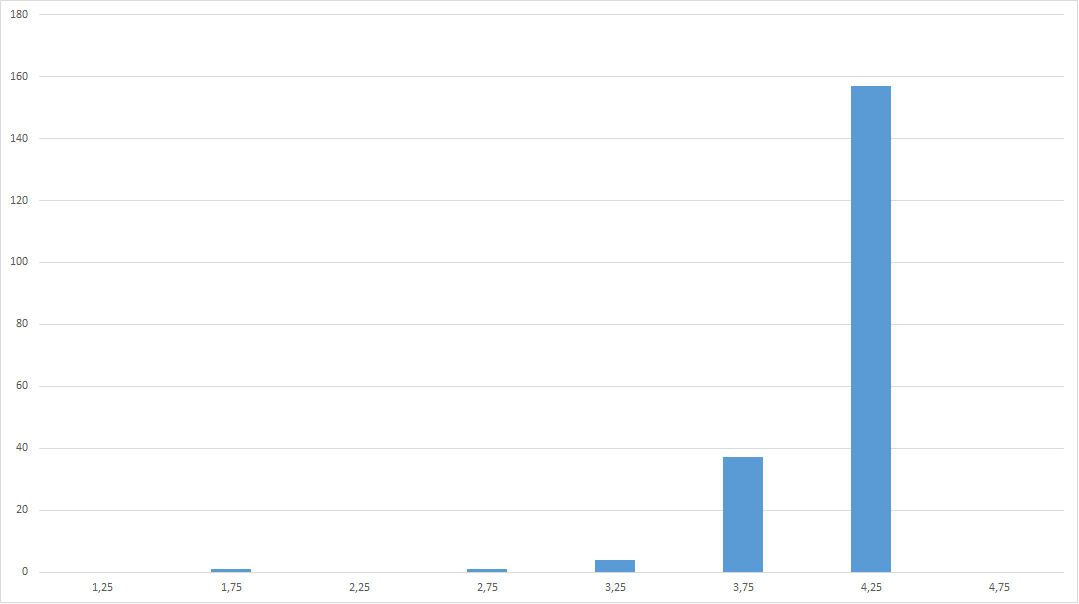
\includegraphics[scale=0.4]{img/histogram.png}
	\caption[Istogramma per il throughput]{Istogramma per il throughput.}
	\label{fig:exp_t_sess}
	\end{center}
\end{figure}

\section{Autocorrelazione}
L'ultima metrica da calcolare è quella relativa all'autocorrelazione. Vediamo sotto forma di tabella i risultati ottenuti per i diversi seed.
\begin{table}[H]
 \centering
 \begin{tabular}{|c|c|c|c|}
 \hline
 \# & SEED: 615425336 & SEED: 37524306 & SEED: 123456789 \\ \hline
 1 & 0,98995668 & 0,98997536 & 0,98994852 \\ \hline
 2 & 0,97981444 & 0,97985091 & 0,97979832 \\ \hline
 3 & 0,96957032 & 0,96962554 & 0,96954728 \\ \hline
 4 & 0,95922107 & 0,95930107 & 0,95919848 \\ \hline
 5 & 0,94876988 & 0,94887862 & 0,94875186 \\ \hline
 6 & 0,93821731 & 0,9383594 & 0,93820573 \\ \hline
 7 & 0,92757015 & 0,92773803 & 0,92755606 \\ \hline
 8 & 0,9168206 & 0,91701647 & 0,91680759 \\ \hline
 9 & 0,90597061 & 0,90619544 & 0,90596156 \\ \hline
 10 & 0,89501832 & 0,89527232 & 0,89501785 \\ \hline
 11 & 0,88396744 & 0,88424369 & 0,88398003 \\ \hline
 12 & 0,87281776 & 0,81311632 & 0,87284494 \\ \hline
 13 & 0,86157167 & 0,86189008 & 0,86161132 \\ \hline
 14 & 0,85022491 & 0,85056456 & 0,85027646 \\ \hline
 15 & 0,83877974 & 0,83913659 & 0,83884245 \\ \hline
 16 & 0,82723641 & 0,82760883 & 0,82730328 \\ \hline
 17 & 0,81559788 & 0,81597844 & 0,81566353 \\ \hline
 18 & 0,80385917 & 0,80424497 & 0,80392133 \\ \hline
 19 & 0,79202286 & 0,79241003 & 0,79208271 \\ \hline
 20 & 0,78008154 & 0,78047206 & 0,78014424 \\ \hline
 \end{tabular}
 \caption{Tabella esperimenti eseguiti per il front-end esponenziale}
 \end{table}
 
 \section{Confronto con altre distribuzioni}
 Il simulatore come già detto offre la possibilità di variare la distribuzione del front-end allo scopo di vedere le possibili variazioni di performance del sistema.
 Le distribuzioni utilizzate sono state le seguenti:
 \begin{itemize}
  \item Esponenziale
  \item 10 Erlang
  \item Iperesponenziale
 \end{itemize}
Per confrontare i vari casi di studio è stato utilizzato il tempo di risposta. In questo caso notiamo come ci sia un peggioramento delle condizioni nel caso la distribuzione usata sia la 10 Erlang, mentre nel caso dell'iperesponenziale abbiamo un comportamento molto simile all'esponenziale.
%\begin{figure}[H]
%	\begin{center}
%	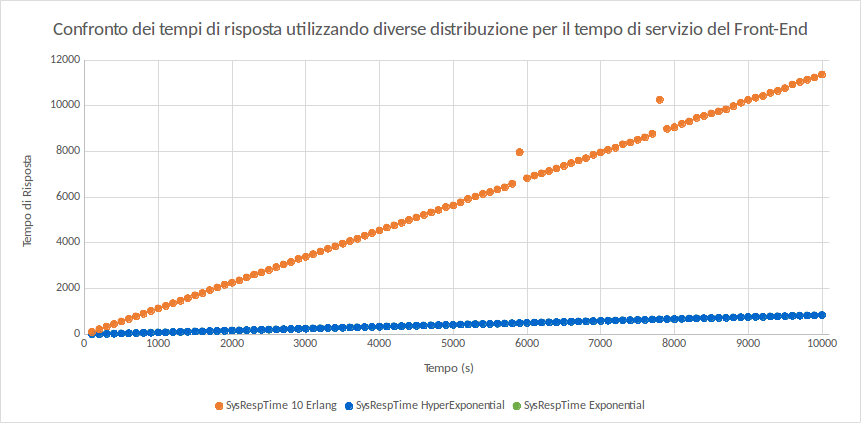
\includegraphics[scale=0.5]{img/confr_distrib.png}
%	\caption[Confronto tra i tempi di risposta]{Confronto tra i tempi di risposta.}
%	\label{fig:confr_distrib}
%	\end{center}
%\end{figure}

\section{Overload manager}
Osservando i risultati conseguiti nella sezione precedente è stato deciso di attivare il meccanismo di overload management sulla distribuzione 10 Erlang. Questo perchè tra le 3 distribuzioni ha mostrato l'andamento peggiore. Si è quindi effettuata una nuova analisi delle metriche prima illustrate.

\subsection{Tempo di risposta}
Il tempo di risposta del sistema quando è attivato questo meccanismo tende a scendere rispetto a prima e risulta arrivare quasi ad una stabilità. Questa stabilità però non è proprio reale in quanto il sistema \textit{oscilla} attorno a questo valore, anche a causa del fatto che le sessioni già accettate vengono abortite.

\begin{figure}[H]
	\begin{center}
	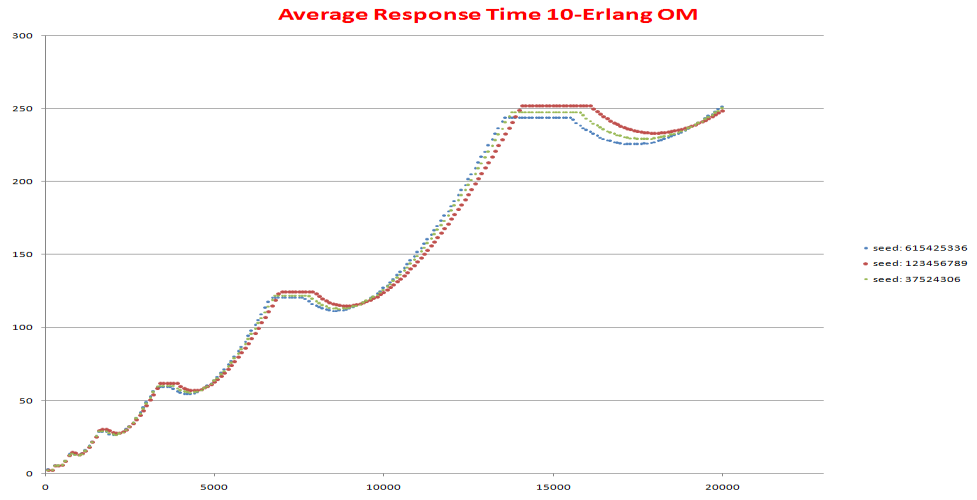
\includegraphics[scale=0.4]{img/er_om_res_time.png}
	\caption[Tempo di risposta del sistema nel caso di una 10 Erlang con overload manager]{Tempo di risposta del sistema nel caso di una 10 Erlang con overload manager.}
	\label{fig:erl_om_res_time}
	\end{center}
\end{figure}

\subsection{Throughput}
\begin{figure}[H]
	\begin{center}
	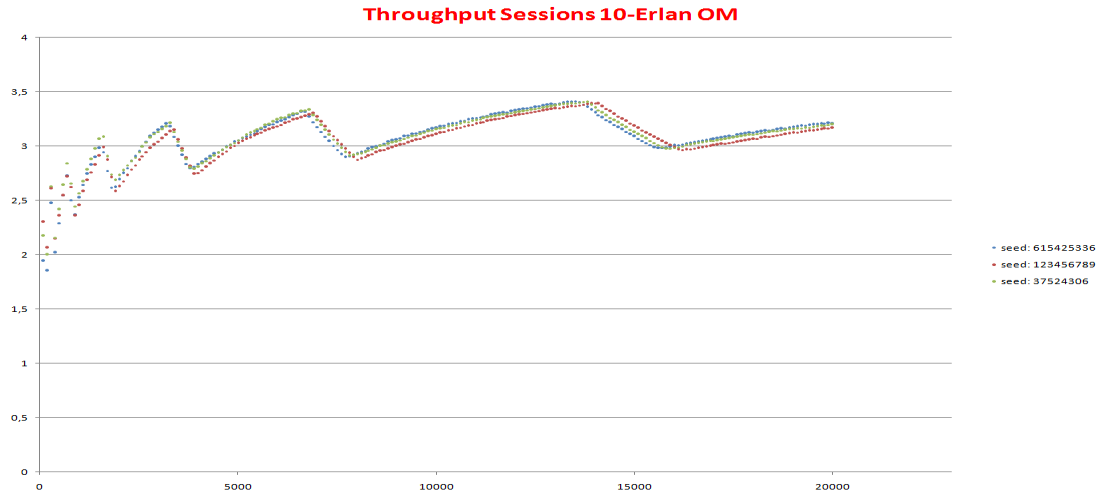
\includegraphics[scale=0.4]{img/erl_om_t.png}
	\caption[Throughput nel caso di una 10 Erlang con overload manager]{Throughput nel caso di una 10 Erlang con overload manager.}
	\label{fig:erl_om_t}
	\end{center}
\end{figure}
Per il throughput osserviamo lo stesso effetto descritto precedentemente in quanto si assesta attorno ad un valore però senza mai fermarsi del tutto, bensì oscillandovi attorno.



\subsection{Drop Ratio}
Il drop ratio misura il rapporto tra le sessioni rifiutate dal sistema e il numero di sessioni totali (ovvero accettate + rifiutate).
Notiamo che questo numero si assesta intorno al 30\% e questo accade poichè vengono rifiutate anche le connessioni già presenti, ciò permette al sistema di scendere molto velocemente sotto il 75\% di utilizzazione e riprendere dunque un normale funzionamento.
\begin{figure}[H]
	\begin{center}
	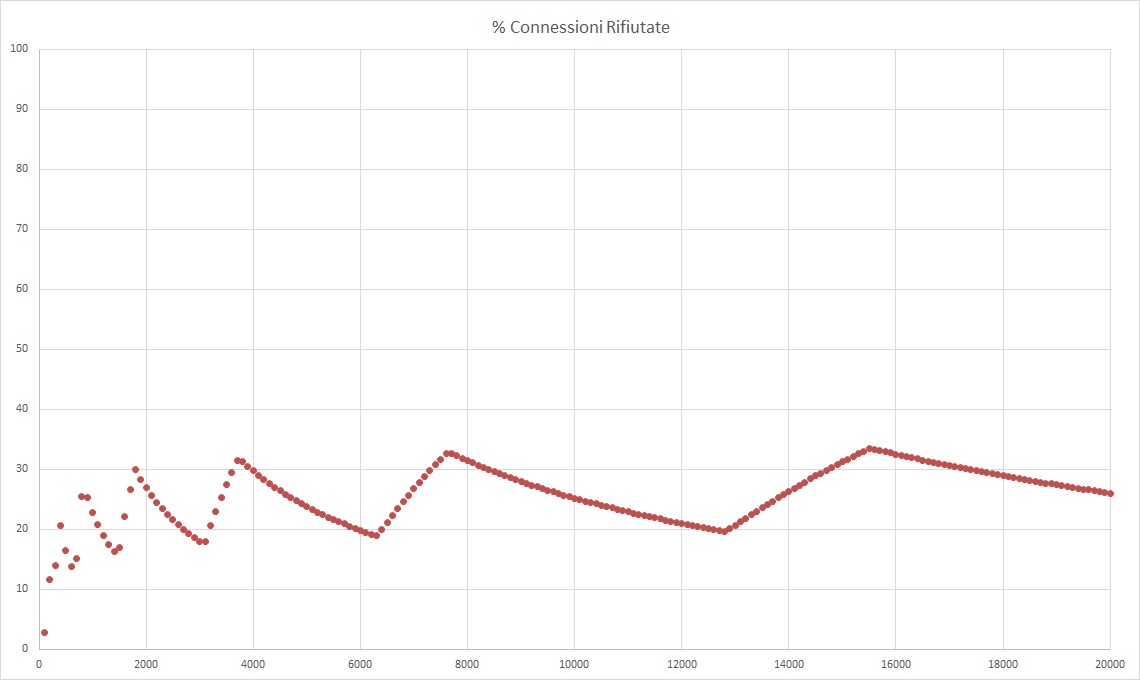
\includegraphics[scale=0.4]{img/Drop_ratio.png}
	\caption[Percentuale di connessioni rifiutate dal sistema.]{Percentuale di connessioni rifiutate dal sistema.}
	\label{fig:confr_distrib}
	\end{center}
\end{figure}

\subsection{Abort Ratio}
Nel caso di overload manager attivo il nostro simulatore deve impedire ad \textbf{ogni richiesta} di potersi mettere in coda al Front Server.
A causa di questo vincolo l'abort ratio è diverso da zero poichè questo si riferisce alle sessioni che vengono chiuse pur essendo state precedentemente accettate dal sistema. Come si può vedere dal grafico la percentuale di connessioni abortite dal sistema è abbastanza elevato.
\begin{figure}[H]
	\begin{center}
	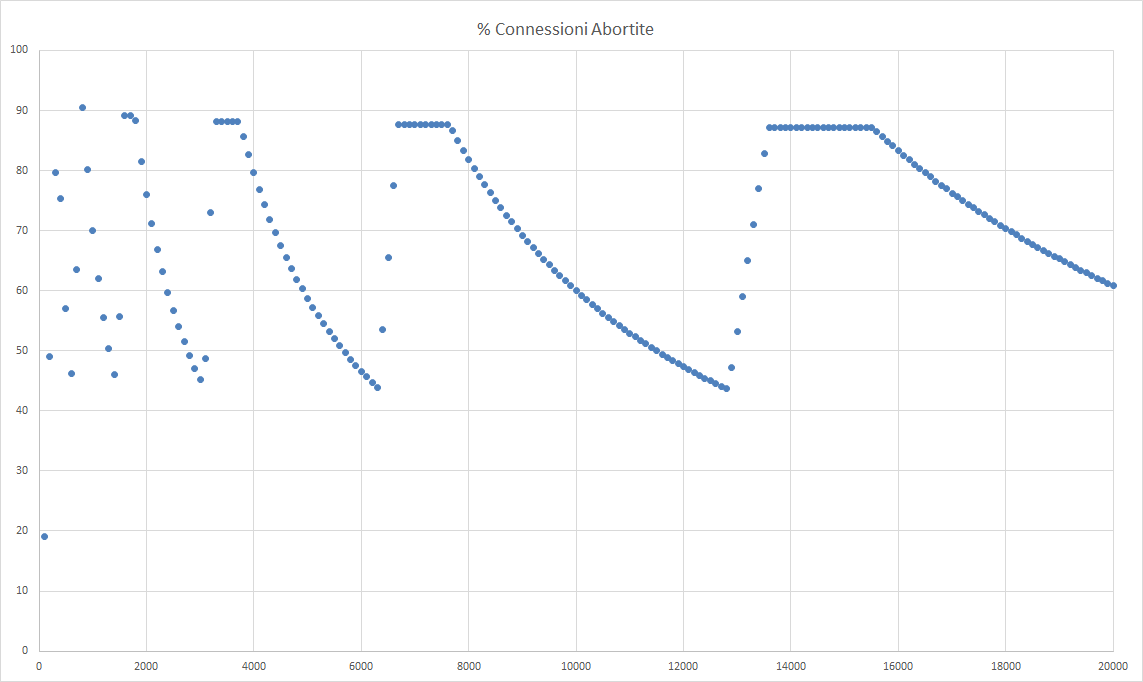
\includegraphics[scale=0.4]{img/abort_ratio.png}
	\caption[Percentuale di connessioni abortite dal sistema.]{Percentuale di connessioni abortite dal sistema.}
	\label{fig:confr_distrib}
	\end{center}
\end{figure}
